\section{Tissue segmentation}

% Implement a Gaussian Mixture Model (GMM) to segment the 20 non-segmented MRI brains and optimise your model through an Expectation-Maximisation scheme [15].

\subsection{Expectation-Maximisation}
In order to perform the tissue classification, an Gaussian Mixture Model (GMM) using Expectation-Maximisation (EM) optimisation algorithm has been implemented following \cite{leemput_automated_1999-1}. The initial version that has been developed receives as input the $T_1$-weighted image and the number of classes. The means and variances of the gaussian functions representing each class are initialised randomly, and scaled using the image values:

\begin{equation}
  \mu_k = [\max(y) - \min(y)] R + \min(y)
\end{equation}
and
\begin{equation}
  \sigma^2_k = a R + b [\max(y) - \min(y)]
\end{equation}
where $\mu_k$ is the mean intensity of class $k$, $y$ is the T1 image, $R$ is a random number between 0 and 1 and $a$ and $b$ are scaling parameters that have been set to 10 and 0.8, respectively.

Once the gaussians parameters have been initialised, the EM loop is run until convergence or until a maximum number of iterations has been reached. The convergence happens when the ratio between the log-likelihood of the current and previous iterations is greater than $1 - \epsilon$, where the convergence threshold $\epsilon$ has been set to $10^{-5}$. The algorithm usually converges around 12 iterations, and the maximum number of iterations has been set to 30. All these parameters are customisable by the user when calling the EM method.

When the EM loop is finished, each voxel is assigned to the class with the highest probability and a label map representing the automatic segmentation is saved. Figure \ref{fig:em-first} shows the results of a segmentation. Since no spatial information is used, the algorithm has assigned voxels outside the brain to be brain tissue, and some voxels are isolated within a different class, which is is not plausible anatomically. Adding TPMs as priors and using Markov random field (MRF) smoothing is necessary to produce a more realistic output.

\begin{figure}
  \centering
  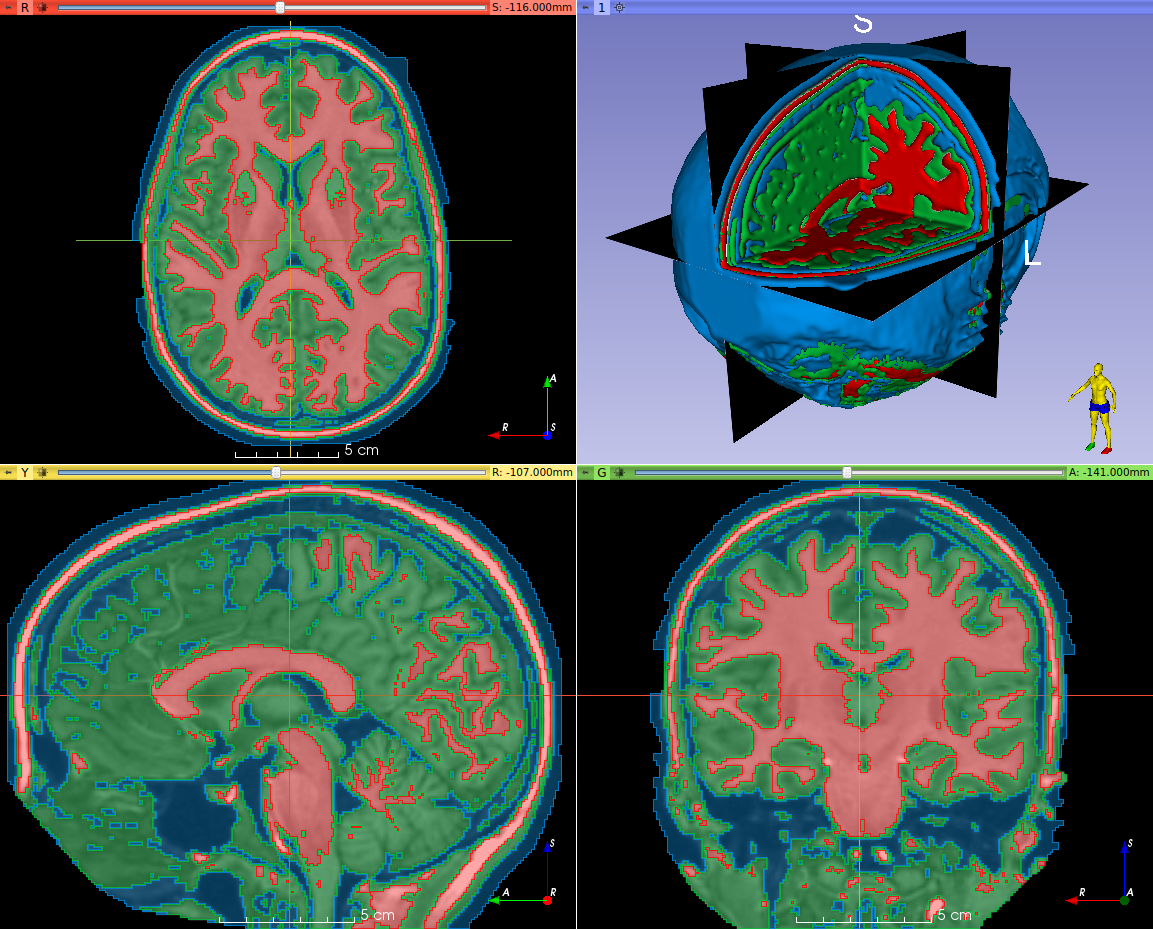
\includegraphics[width=0.7\textwidth]{figures/em_first}
  \caption{Results of an automatic segmentation. Aproximate classes are: blue - CSF; green - GM; green - WM. The Dice scores compared to the provided segmentation are: 0.38 for CSF, 0.66 for GM and 0.73 for GM.}
  \label{fig:em-first}
\end{figure}

The uncertainty of the algorithm assigning a voxel $i$ to a class can be measured as $u_i = 1 - \sigma_i$. Figure \ref{fig:em-first-uncertainty} shows the uncertainty for the segmentation of Figure \ref{fig:em-first}. The most certain zones are the background and the inner parts of the WM, while the most uncertain ones are the interfaces between different tissues. TODOOOOOOOOOOOOOOOOO

% Use image registration to propagate the previously generated tissue probability maps into the space of the non-segmented brain MRIs. This can be achieved by registering the groupwise mean template to the non- segmented brain and then applying the obtained transformation to the probability maps.


% Use then the propagated probability maps as a priori information in your GMM [10]. If you did not complete the previous section, you may use the provided prior files.

% Embed a Markov random field into your segmentation framework to introduce a spatial smoothness term in the label estimation process [10].

% MRI acquisition usually suffers from intensity non-uniformity (INU), improve the robustness of your GMM framework to INU by adding a bias field correction component to the probabilistic model [5].

% Describe each component of your GMM framework in the report and motivate their use.

% Use one already segmented images to optimise your implementation parameters (e.g. INU complexity, MRF beta term) [10].

% By choosing these parameters, bias can be introduced in the optimisation. Describe one potential bias and propose a solution to avoid it [5]?
